% Author: Pavol Loffay
% Project: Master thesis - Hawkular alert prediction
% Date 20.2.2015

\chapter{Introduction}
In driving successful business on the internet it is important to assure an application
health and reliability. One can achieve that by monitoring subjected resources and setting
up a clever alerting system. These features are offered in many monitoring systems, however 
being predictive in this area can even prevent undesirable states and most importantly gives administrators more time for
reacting to such events. For instance it can decrease downtime of an application 
or ability to load balance workload in advance by horizontal scaling targeted services. 

As alerting system are sophisticated and can be composed by many conditions so this work
focuses only on predicting future metrics values which are then sent as input to an alerting system. 

In the first chapter are discussed various approaches for time series modeling and
forecasting. Second chapter focuses on implemented models with validation on real and 
generated test data sets. Implementation details with testing can be found in fourth chapter.

TODO describe chapters

    \section{Hawkular}
    The implementation part of the master's thesis is developed as a part of an open source project
    Hawkular\footnote{Available at \url{http://www.hawkular.org}}. 
    Therefore the application architecture and used technologies had to fit 
    into the overall project architecture.

    Hawkular is middleware monitoring and management platform
    developed by company Red Hat and independent community of contributors.
    It is a successor to very successful RHQ\footnote{Available at \url{https://rhq-project.github.io/rhq/}} 
    project, also known as JBoss Operations Network (JON).
    By monitoring is meant that there are agents for diverse applications which
    push data to the server. These agents can also execute application specific actions. 

    The monolithic architecture of RHQ project was due it's size hard to maintain 
    and lacking robust REST api lead to fresh development of new application.   
    In contrast Hawkular consist of several loosely coupled or even independent applications.
    These independent components are much
    easier to maintain and more importantly they communicate over REST api. This
    architecture of microservices and chosen protocol allow simple development of 
    agents which can be written in any programming language. In RHQ only Java agent were
    available. Hawkular as product is customized Wildfly
    \footnote{An open source project of JBoss EnterpriseApplication Platform.}
    application server with all components deployed in it.

    \begin{itemize}
        \item Console\,--\,user web interface
        \item Accounts\,--\,authorization subsystem based on Keycloak\footnote{An open
            source single sing-on and identity management for RESTful web services.}
        \item Inventory\,--\,graph based registry of all entities in Hawkular
        \item Metrics\,--\,time series metrics engine based on Cassandra\footnote{An open
            source distributed database management system. Hybrid between key\,--\,value and
        column\,--\,oriented database.}
        \item Alerts\,--\,alerting subsystem based on JBoss Drools
    \end{itemize}

    Some of the modules uses also Java messaging topics (JMS) for inter\,--\,component
    one to many communication.

    Modules are packaged as standard Java web archives (WAR), or enterprise archives (EAR)
    and deployed into customized Wildfly. Build and package management is performed by 
    Maven and Gulp for user interface modules. 

    \section{Data Mining Goals}
    The goal of this thesis is to develop module for Hawkular which will provide forecasts for any 
    time series metrics collected by agent. On new metric data available the module
    learns from data and predicts new values. Based on this predicted values an alert can
    be triggered. Forecast should be also available for user interface in predictive
    charts. 

    One Wildfly agent on average collects hundreds to thousands metrics, therefore module
    should be capable of processing high volume of data. Some of the customers monitor
    hundreds of server each with multiple agents. Therefore performance of chosen 
    learning algorithm has to be taken in account.

%%%%%%%%%%%%%%%%%%%%%%%%%%%%%%%%%%%%%%%%%%%%%%%%%%%%%%%%%%%%%%%%%%%
\chapter{Time Series Models} \label{models}
This chapter focuses on time series theory and various approaches for modelling time series.
Models are ordered from simpler to more complex ones. 

Firstly, it is important to define time series; it is sequence of observations
$s_t \in \mathbb{R}$ ordered in time. This thesis focuses only on univariate equidistant 
discrete time series. Time series analysis contains many segments, this work focuses on 
forecasting. It is defined as a process of making prediction of the future based 
on the past. In other words, forecasting is possible because  
future depends on the past or analogously because there is a relationship
between the future and the past. However, this relation is not deterministic and 
can be hardly written in an analytical form.

There are two forecasting types: qualitative and quantitative.
Qualitative methods are mainly based on the opinion of the subject and are used 
when past data are not available, hence not suitable for this project. 
If there are past data available, quantitative forecasting methods are more suitable. 

TODO mention that we talk only about models which makes sense to use in our environment.

    %%%%%%%%
    \section{Simple quantitative methods}
    Following methods are the simples forecasting quantitative models. They can be used on
    any time series without further analysis. 

    \begin{itemize}
        \item Average method\,--\,forecasts are equal to the value of the mean of
            historical data.
            \begin{eqnarray}
                \hat{y}_{T+h|T} = \overline{y} = (y_{1}+ \dots + y_{T}) / T 
            \end{eqnarray}
        \item Na\"{i}ve method\,--\,forecasts are equal to the last observed value.
            \begin{eqnarray}
                \hat{y}_{T+h|T} = y_{T}
            \end{eqnarray}
        \item Drift method\,--\,variation of na\"{i}ve method which allow the
            forecasts to increase or decrease over time.
            \begin{eqnarray}
                \hat{y}_{T+h|T} = y_{T} + \frac{h}{T-1} \sum_{t=2}^T{y_{t} - y_{t-1}} = 
                    y_{T} + h(\frac{y_{T}-y_{1}}{T-1}) 
            \end{eqnarray}

    \end{itemize}
    There is also a seasonal variant of na\"{i}ve model. This method is suitable only
    for highly seasonal data. These methods in general produces high forecasting error 
    but are very easy to implement.

    %%%%%%%%
    \section{Linear Regression}
    Linear regression is classical statistical analysis technique. It is often used to
    determine whether there is linear relationship between dependent and eventually more
    independent variables. It is also often used for predictions mainly in econometric
    field. 

    Simple linear regression is defined as:
    \begin{eqnarray}
        y = \beta_0 + \beta_1 x + \epsilon
    \end{eqnarray}

    Parameters $\beta_0$ and $\beta_1$ are calculated by minimizing the sum of squared
    errors:
    
    \begin{eqnarray}
        SSE = \sum_{i=1}^N \epsilon_{i}^2 = \sum_{i=1}^N (y_i - \beta_0 - \beta_1 x_i)^2
    \end{eqnarray}
    
    Once parameters are estimated predictions for any time in the future can be calculated. 
    If modelled time series is not stationary then and for instance trend changes over
    time parameters has to be periodically estimated to achieve better accuracy. 
    %For econometric analysis it is important to use best linear unbiased estimator,
    %where couple of assumptions has to hold:
    %\begin{enumerate}
    %    \item $E(Y_i) = \beta_0 + \beta_1 X_i$
    %    \item $var(Y_i)=\sigma^2$\,--\,homoscedasticity
    %    \item $cov(Y_i, Y_j)=0$, for $i \neq j$
    %    \item $Y_i$ cames from normal distribution
    %    \item $X_i$ is not random variable
    %\end{enumerate}
    %Where $i$ takes values from $1$ to the number of observed values. These assumptions 

    %%%%%%%%
    \section{Simple Exponential Smoothing}
    The concept behind simple exponential smoothing is to attach 
    larger weights to the most recent observations than to observations from distant
    past. Forecasts are calculated using weighted averages where the weights 
    decrease exponentially as observations come from further in the past.
    In other words smaller weights are associated to older observations.
    Equation for simple exponential smoothing is listed in \ref{exp_smoothing}.

    \begin{eqnarray} \label{exp_smoothing}
         \hat{y}_{T+1|T} = l_t \\ \nonumber
         l_t = \alpha y_t + (1-\alpha)l_{t-1}
    \end{eqnarray}

    For smoothing parameter $\alpha$ holds $ 0 \leq \alpha \leq 1 $. Note, if $\alpha = 1$ then \\
    $\hat{y}_{T+1|T} = y_{T}$ so forecasts are equal to the na\"{i}ve method.
    If the parameter $\alpha $ is smaller more weight is given to observations from distance
    in past. 

    Simple exponential smoothing has flat forecast function, that means all forecasts
    all the same. Smoothing can be generally used as technique to separate signal and noise.
    This method is useful if a series does not contain any trend or one is interested only
    in one step ahead prediction. Multi step ahead predictions for time series with trend
    can produce high error.

    %%%%%%%%
    \section{Holt's Liner Trend Method}
    Simple exponential smoothing can be extended to allow forecasting of data with a trend. 
    This was done by Charles C. Holt in 1957. This method is slightly more complicated than 
    original one without trend. In order to add trend component another equation has to be added. 

    \begin{eqnarray} \label{exp_holt}
        \hat{y}_{t+h|t} = l_{t} + hb_{t} \\ \nonumber
         l_t = \alpha y_t + (1 - \alpha) (l_{t-1} + b_{t-1}) \\ \nonumber
         b_t = \beta (l_t - l_{t-1}) + (1 - \beta)b_{t-1} 
    \end{eqnarray}

    Where a parameter $b_t$ denotes a slope of the series and the parameter $l_t$ level. 
    There is also a new parameter smoothing parameter of the slope\,--\,$\beta$. 
    It's rage is equal to $\alpha$, so $\alpha,\beta \in \interval[{0,1}]$. 

    %%%%%%%%
    \section{Holt\,--\,Winters Seasonal Method}
    This method is an extension of Holt's linear trend method with added
    seasonality. It is also called triple exponential smoothing. In this model 
    there are three equations \ref{exp_holt_winters}. 
    One for level, second for trend and third for seasonality.
    Each pattern uses smoothing constant $ \alpha,\beta,\gamma \in \interval[{0,1}]$.

    \begin{eqnarray} \label{exp_holt_winters}
        \hat{y}_{t+h|t} = l_{t} + hb_{t} + s_{t+h_m-m}\\ \nonumber
        l_t = \alpha (y_t - s_{t-m}) + (1 - \alpha) (l_{t-1} + b_{t-1}) \\ \nonumber
        b_t = \beta (l_t - l_{t-1}) + (1 - \beta)b_{t-1} \\ \nonumber
        s_t = \gamma (y_t - l_{t-1} - b_{t-1}) + (1-\gamma)s_{t-m}
    \end{eqnarray}

    Where $h_m=[(h-1) \mod m] + 1$, which ensures that the estimates of the seasonal
    indices came from the correct season. This model can be used only if the period 
    of time series is know beforehand. In Hawkular the period of the time series is 
    unknown, therefore period identification should be also implemented.
    
    %%%%%%%%
    \section{Box\,--\,Jenkins Methodology (ARIMA)}
    Models from Box\,--\,Jenkins methodology are the most widely used in time series
    analysis specially for econometric data. This methodology is based on analysis of autocorrelation (ACF)
    and partial autocorrelation (PACF) functions.
    
    The most generic model is ARIMA(p, d, q). It combines together autoregressive, integrated and
    moving average models. An autoregressive model (AR) consist of sum of weighed lagged observations. It is listed
    in \ref{ar_model}. The order of this model is defined by $p$ and can be determined from PACF function \cite{cipra}.
    A moving average model (MA) is sum of weighted errors of order $q$. The order of this part can be
    determined from ACF function \cite{cipra}. The last part of the model is used when a time series is non stationary.
    There are several ways how to make a  particular time series stationary. Box Jenkins methodology uses
    differencing\,--\,integration part. The order if differencing original series is denoted by $d$ letter. Usually
    first order differences are enough to make time series stationary.

    Parameters of the model, including AR and MA part can by estimated by non-linear
    least squares or maximum likelyhood estimation \cite{brockwell}. For successful estimation a certain number of
    historical points needs to be available. In \cite{cipra} minimal training size is set to at least fifty
    observations.

    \begin{eqnarray} \label{ar_model}
        y_t = \phi_1 y_{t-1} + \phi_2 y_{t-2} + \dots + \phi_p y_{t-p} + \epsilon_t \\ \nonumber
        \epsilon_t \overset{iid}{\sim} N(0, \sigma^2)
    \end{eqnarray}

    Moving averages model should not be confused with simple moving average which is
    used for trend estimation. In moving average model MA(q) the current value is
    a regression against white noise of prior values of the series \cite{wiki-ma-model}. A random noise from
    each point is assumed to come from the same distribution which typically is 
    a normal distribution. Model of the order $q$ is listed in \ref{ma_model}.

    \begin{eqnarray} \label{ma_model}
        y_t = \theta_1 \epsilon_{t-1} + \theta_2 \epsilon_{t-2} + \dots + \theta_p y_{t-q} + \epsilon_t \\ \nonumber
        \epsilon_t \overset{iid}{\sim} N(0, \sigma^2)
    \end{eqnarray}

    It is important mention that models AR(p) and MA(q) are invertible.
    Therefore any stationary AR(p) model can be written as MA($\infty$) and with some assumptions
    vice versa \cite{brockwell}. ARIMA model is often written with backshift operator $By_t=y_{t-1}$.
    With this operator ARIMA(p, d, q) is listed in \ref{arima}. On the left side of the equation is AR(P) process
    and on the right MA(q).

    \begin{eqnarray} \label{arima}
        (1- \phi_1B - \dots - \phi_pB^p)(1-B)^d y_t = \\ \nonumber
         c + (1+\theta_1B+\dots+\theta_qB^q) \epsilon_t
    \end{eqnarray}

    After this theoretical part it is clear that ARIMA models are more complicated than family of moving averages.

    %%%%%%%%
    \section{Artificial Neural Networks}
    Recently a large number of successful applications using neural networks for time series modeling show that they
    can produce valuable results \cite{ann-forecasting-state-art}. There are several non trivial issues with
    determining the appropriate architecture of the network. This has to be taken into account because it can
    dramatically effect learning performance and forecasting accuracy \cite{ann-model-selecting}.
    Besides the problems with selecting right architecture learning process of artificial neural network is much more
    computationally expensive than selecting appropriate ARIMA or exponential smoothing model \cite{ann-forecasting}.

    Because Hawkular forecasting engine should be capable of predicting thousands of metrics at the same time, models
    based on neural networks would have too high computational requirements. Therefore they are not suitable for our
    environment.

    %%%%%%%%
    \section{Time series decomposition}
    In modelling time series it is sometimes necessary to decompose series to trend, seasonal and random component
    \cite{otexts}. It is also used for initialization seasonal indices in triple exponential smoothing.

    \begin{itemize}
        \item \textbf{Trend $ T_{t} $}\,--\,exists if there is long term increase or decrease over
            time. Can be linear or nonlinear (e.g. exponential growth)
        \item \textbf{Seasonal $ S_{t} $}\,--\,exists when a series is influenced by seasonal factors.
            Seasonality is always of fixed and known period.
        \item \textbf{Cyclic $ C_{t} $}\,--\,exists it there are long term wave-like patterns.
            Waves are not of a fixed period.
        \item \textbf{Irregular $ E_{t} $}\,--\,unpredictable random value referred as white
            noise. 
    \end{itemize}

    Decomposition can be written in many forms. Two of them are additive and multiplicative \ref{decomposition}.
    Which one to use depends on the underlying time series model.

    \begin{eqnarray} \label{decomposition}
        y_{t} = T_{t} + S_{t} + C_{t} + E_{t} \\
        y_{t} = T_{t} \times S_{t} \times C_{t} \times E_{t}
    \end{eqnarray}

    An algorithm for additive decomposition consist of following steps:

    \begin{itemize}
        \item Compute a trend component $\hat{T}_t$ using moving average model. If a period is even use
        $2 x MA(period)$. If period is an odd number use $MA(period)$. $2 x MA$ for even period is used because it
        has to be symmetric.
        \item Calculate detrended series $y_t - \hat{T}_t$.
        \item Estimate seasonal indices $\hat{S}_t$ for each period by averaging values of given period. For example,
         the seasonal index for Monday is the average for all detrended Monday values in the data. Then the mean of
         seasonal indices is subtracted from each period.
        \item Random component is calculated by subtracting trend and seasonal component from original time series
            $\hat{E}_t = y_t - \hat{T}_t - \hat{S}_t$.
    \end{itemize}

    %%%%%%%%
    \section{Augmented Dickey\,--\,Fuller Test}
    Time series statistical tests are often used for testing if there is particular characteristics present in time
    series. Unit root test are used whether a time series in non stationary. In this work Augmented Dickey\,--\,
    Fuller (ADF) test was chosen for unit root testing. It's null hypothesis $H_0$ is time series contains a
    unit root \,--\, it is not stationary. Outcome of this test is a negative ADF statistics. The more negative it is
    the stronger the rejection of the hypothesis. The full form of ADF test is listen in \ref{adf-test}.

    \begin{eqnarray} \label{adf-test}
        \Delta y_t = \alpha + \beta t + \gamma \Delta y_{t-1} + \dots + \delta{p-1} \Delta y_{t-p+1} + \epsilon_t \\
        ADF = \frac{\hat{\gamma}}{SE(\hat{\gamma})} \label{adf-stat}
    \end{eqnarray}

    There are multiple variants of ADF test. Some of them leave out some parts of equation \ref{adf-test}.
    The most important ones and widely used are:

    \begin{itemize}
        \item \emph{nc}\,--\,no constant - for regression with no constant not time trend ($\beta t$)
        \item \emph{c}\,--\,constant for regression with an intercept but no time trend ($\beta t$)
        \item \emph{ct}\,--\,for a regression with an intercept and time trend
    \end{itemize}

    Each of them is good for testing particular type of stationarity. For example for testing if there is time trend
    present in the time series \emph{c} version is best choice.

    The implementation of this test is to fit multiple linear regression model of equation \ref{adf-test}. Then
    calculate ADF statistics with \ref{adf-stat}. SE denotes standard error of estimated $\hat{\gamma}$.

    %%%%%%%%
    \section{Seasonality detection}
    Forecasting engine in Hawkular system does not have any inside information of period of a time series being
    modelled. Therefore automatic period identification has to be implemented. In practice it is
    a difficult task and result often differs from correct period, specially if there is significant noise present in
    the series \cite{period-meteo}.

    There are several ways how to implement automatic period identification. The most used ones are based on
    autocorrelation function (ACF) or spectral density \cite{period-hydman}. This work applies ACF method.
    In the following chart \ref{img:period-acf} ACF function of sine function is shown. The period of this
    function is seven. There are patterns repeated every seven observations and it is decreasing to zero.

    \begin{figure}[H]
        \begin{center}
            \scalebox{0.5}{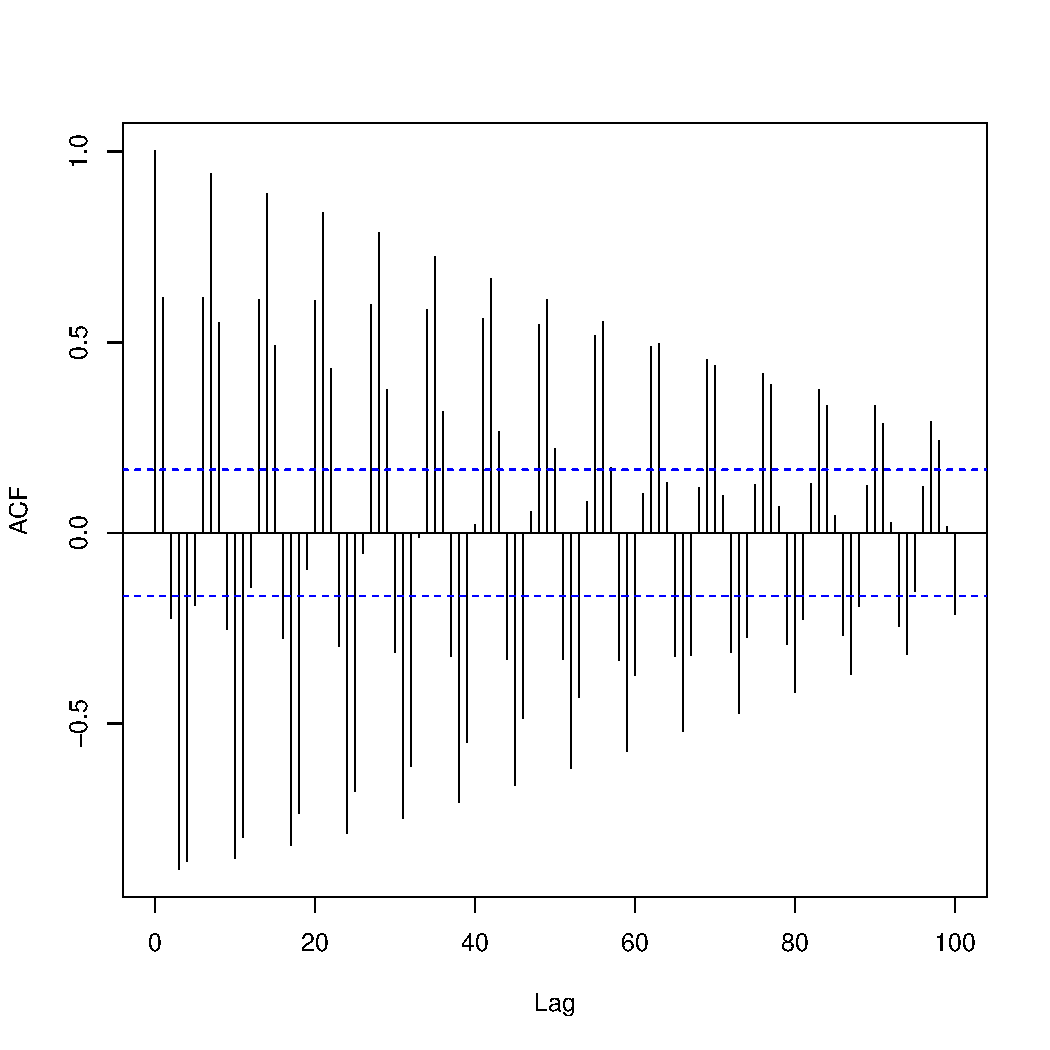
\includegraphics{img/acf-sine.pdf}}
            \caption{ACF of sine function.}
            \label{img:period-acf}
        \end{center}
    \end{figure}

    The algorithm for automatic period identification is demonstrated in \ref{alg:period-find}. It uses ACF function
    It is looking for periodically significant values of ACF function. These values have to be decreasing to zero at
    some rate. At the infinity lag ACF approach zero.

    The algorithm first calculates autocorrelation function of input time series and it finds index of the highest
    value. Follows \texttt{checkPeriodExists} where it checks if there are significant values of ACF present at following $n*period$
    indices of autocorrelation function. There have to be present at lease two consecutive values of ACF, so $n$ takes
    values from $1,2,3\dots$

    \begin{algorithm}
        \caption{Find period of time series} \label{alg:period-find}
        \begin{algorithmic}[1]
        \Function{findFrequency}{$int[] ts$}
            \If{$unitRootPresent(ts)$} \Comment{e.g. ADF test}
                \State $ts \gets diff(ts)$ \Comment{first order differences}
            \EndIf
            \State $acf \gets acf(ts)$ \\
                        \Comment{returns index of the highest value}
            \State $period \gets findHighest(ts, period)$
            \While{$period * 2 < ts.length$}
                \If{$checkPeriodExists(x, ts)$}
                    \State \Return $period$
                \EndIf
                $period \gets findHighest(ts, period)$
            \EndWhile
            \State \Return $0$
        \EndFunction
        \end{algorithmic}
    \end{algorithm}

    %%%%%%%%
    % \section{Optimization Algorithms}
    % TODO

%%%%%%%%%%%%%%%%%%%%%%%%%%%%%%%%%%%%%%%%%%%%%%%%%%%%%%%%%%%%%%%%%%%
\chapter{Models Demonstration}
In the previous chapter several models for forecasting were discussed, however in Hawkular only a few of them were
selected and implemented. It is because various time complexity of the models and more important robustness in terms of
beeing able to produce accurate results for higher range of modelled time series.
Following model evaluations and graphs are generated using statistical system R.

    %%%%%%%%
    \section{Metrics in Hawkular}
    In Hawkular there are three types of metrics: gauge, counter and availability. All of them are univariate metrics
    of structure \\$\{timestamp, value\}$. Each of these types is used for collecting dedicated types of metric data.
    For example gauge can increase or decrease over the time, counter is monotonically decreasing or increasing and
    availability represents up or down state of a resource.

    %%%%%%%%
    \section{Evaluating Forecasting Accuracy}
    In order to evaluate model it is important to estimate an error of the forecast. There are 
    several statistics for evaluating forecasting errors. The most used ones are mean squared error (MSE)
    \ref{accuracy-mse} and mean absolute error (MAE) \ref{accuracy-mae}. The difference between them is that MSE
    emphasizes the extremes while MAE is more robust to outliers.

    \begin{subequations} \label{accuracy}
        \begin{align} \label{accuracy-mse}
             MSE = \frac{1}{n} \sum_{i=1}^{n}(y_i - \hat{y_i}) \\ \label{accuracy-mae}
             MAE = \frac{1}{n} \sum_{i=1}^{n} \abs{y_i - \hat{y_i}}
         \end{align}
    \end{subequations}

    %%%%%%%%
    \section{Model Selection} \label{model-selection}
    When comparing multiple models, statistics like MSE or MAE are not the best objective functions. Comparison
    based on this statistics can select complicated model with lots of parameters, which may overfits training data
    and most importantly it selects less robust model \cite{cipra}. Therefore for comparing multiple models another
    factors has to be added to the objective function. These factors are number of parameters of the model. The
    most used criteria for model sections are: Akaike information criterion (AIC) and Bayesian information
    criterion (BIC). Model with lower information criterion is preferred.

    \begin{eqnarray} \label{aic}
        AIC = 2 k - \ln(L) \\ \nonumber
        BIC = k \ln(n) - 2 \ln(L)
    \end{eqnarray}

    Equations for AIC and BIC are listed in \ref{aic}. Number of parameters of the model represents $k$, $n$ is number
    of observations and $L$ is maximized value of the likelihood function of the model. In case for exponential
    smoothing it is minimized sum of squared error of one step ahead prediction of training data set. From the
    equations it can be seen that BIC penalizes models with more parameters. There is also AIC criterion with
    correction form \ref{aicc}. Corrected version of AIC more penalizes longer models.

    \begin{eqnarray} \label{aicc}
        AICc = AIC + \frac{2k(k+1)}{n-k-1}
    \end{eqnarray}

    %%%%%%%%
    \section{Evaluation on Data}
    An analytical process of modelling time series advise to plot the data and fit various models chosen by an
    forecaster previous experience. In second step compare statistics of those models and choose one the best describes
    data. However, this approach can be used only if a process of modelling is conducted by human being.

    In this section a real time series is modelled using time series discussed in section \ref{models}.
    Chosen time series is \emph{austourists} from R package \texttt{fpp}. This series is a measurement of quarterly
    visitor nights spent by international tourists in Australia. It was chosen on purpose because it
    contains trend and seasonality.

    In the first chart \ref{img:simple-models} there is depicted na\"{i}ve, average and drift model. Average model is
    just an overall average of the whole time series. It does not change over time. However there could be online
    version of this algorithm for which an average would be calculated for each new value. Na\"{i}ve and drift model
    copy values of time series with one step lag. These two models differs in forecasts. Drift model is capable of
    capturing trends.

    \begin{figure}[H]
        \begin{center}
%            \resizebox{12cm}{8cm}{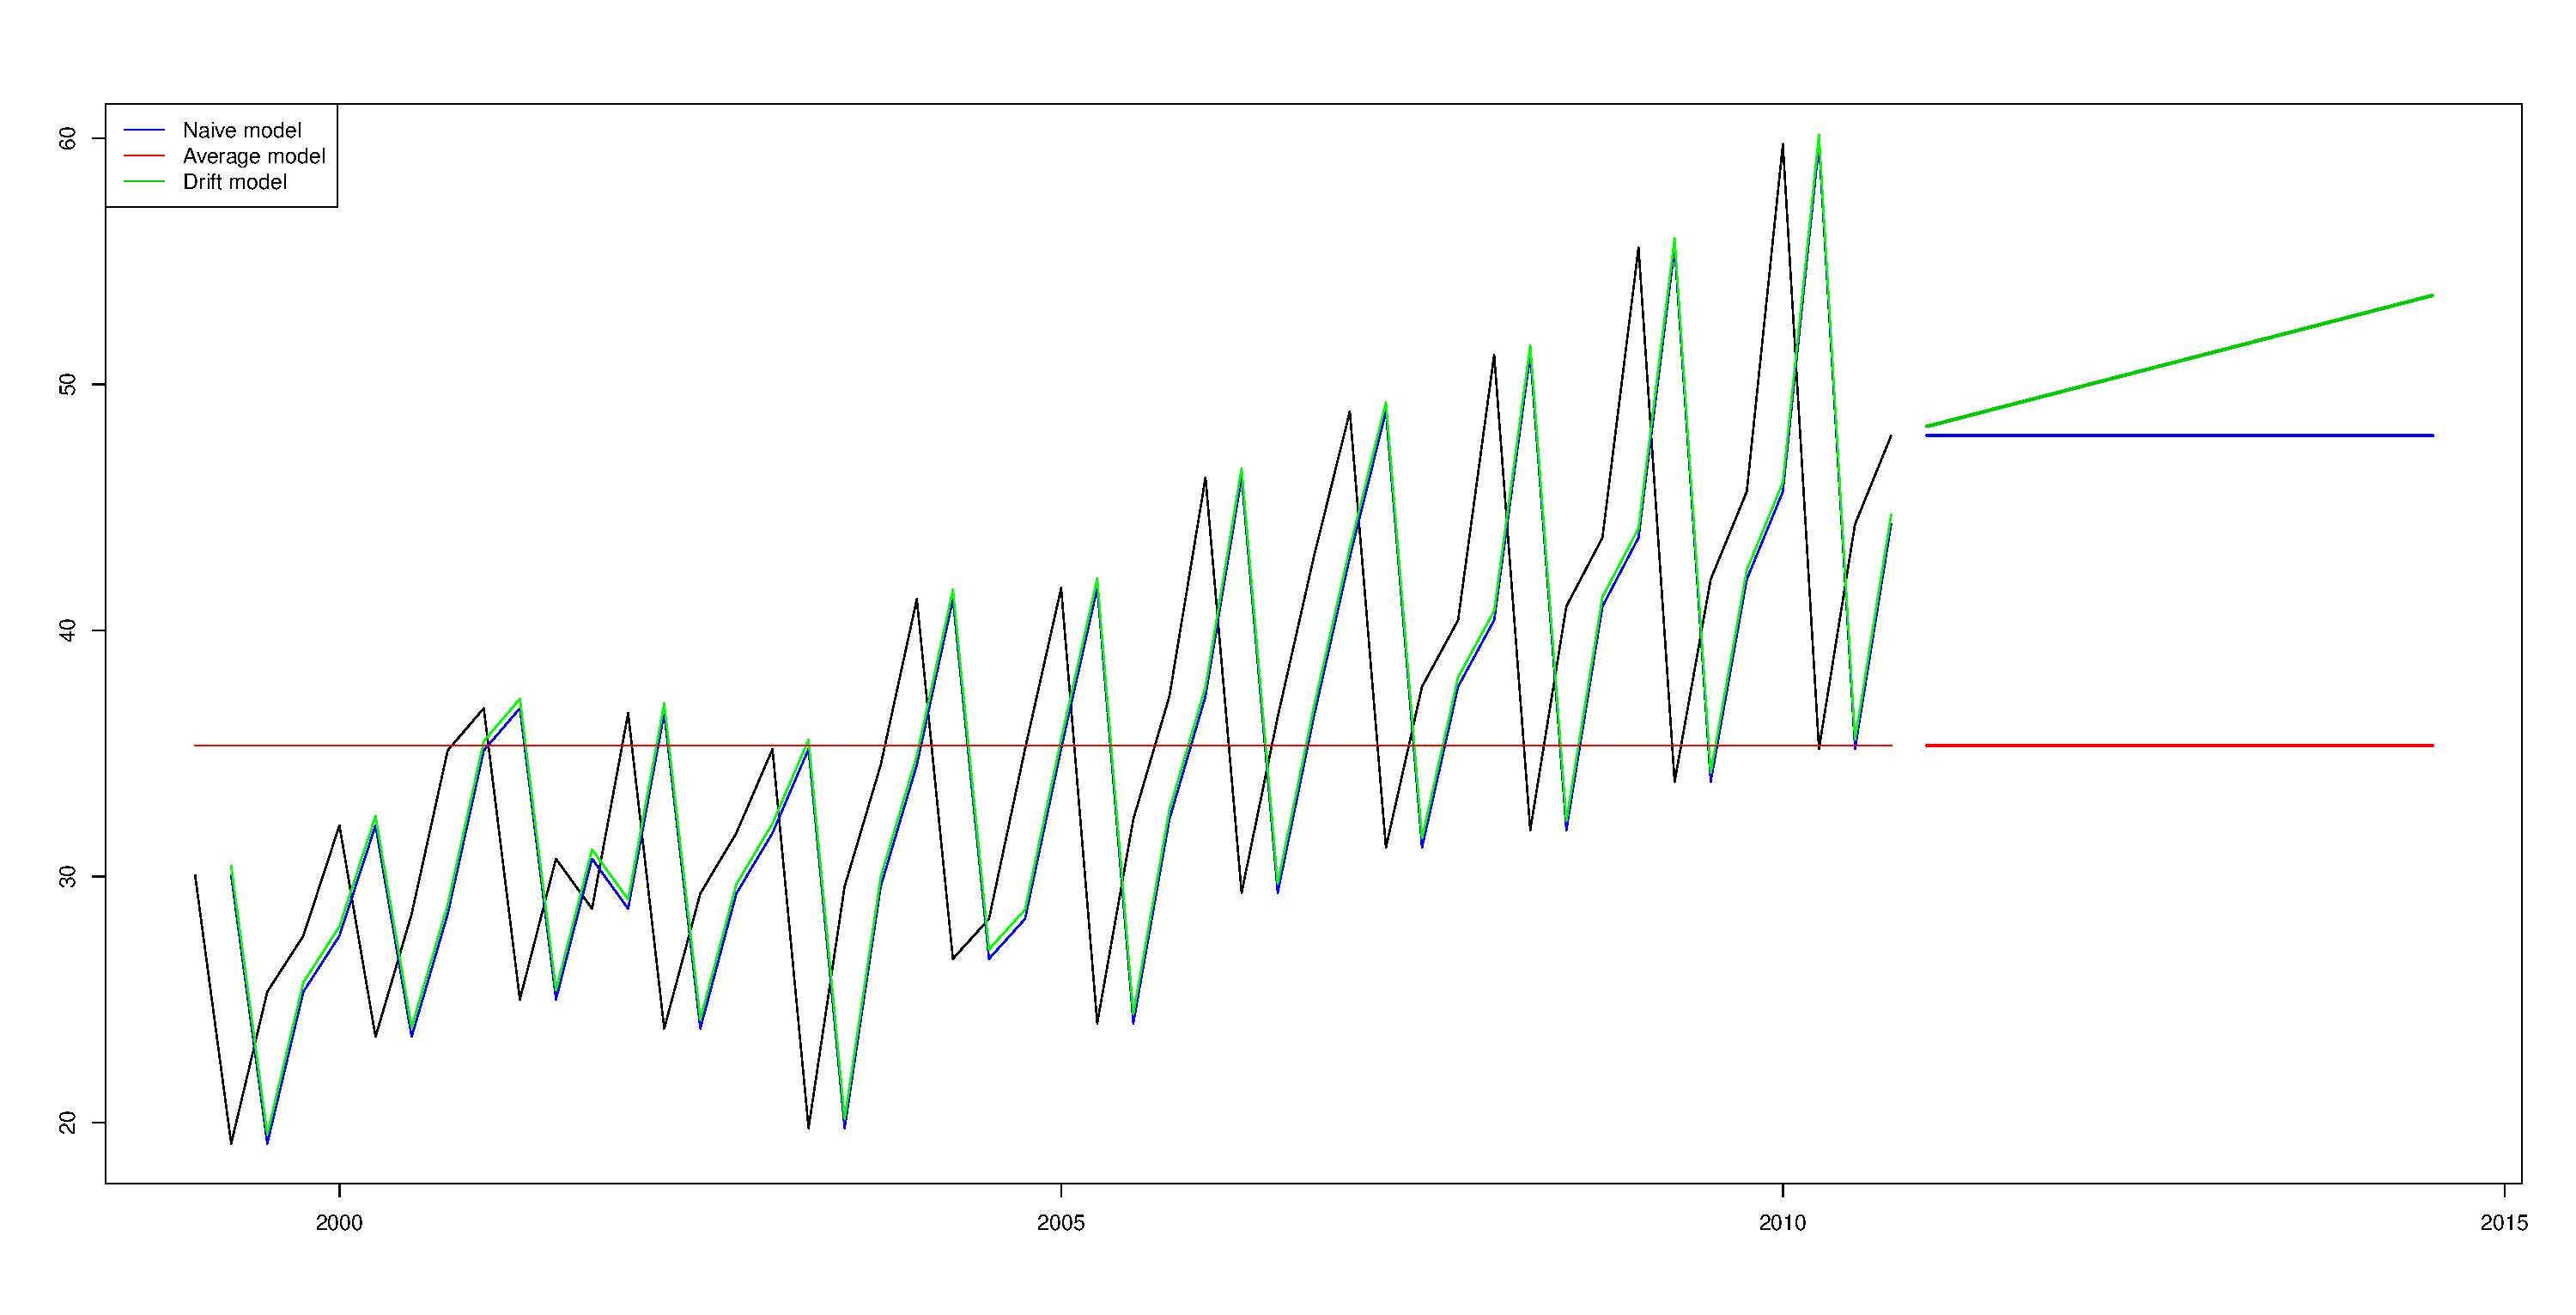
\includegraphics{img/simple-models.pdf}}
            \scalebox{0.25}[0.2]{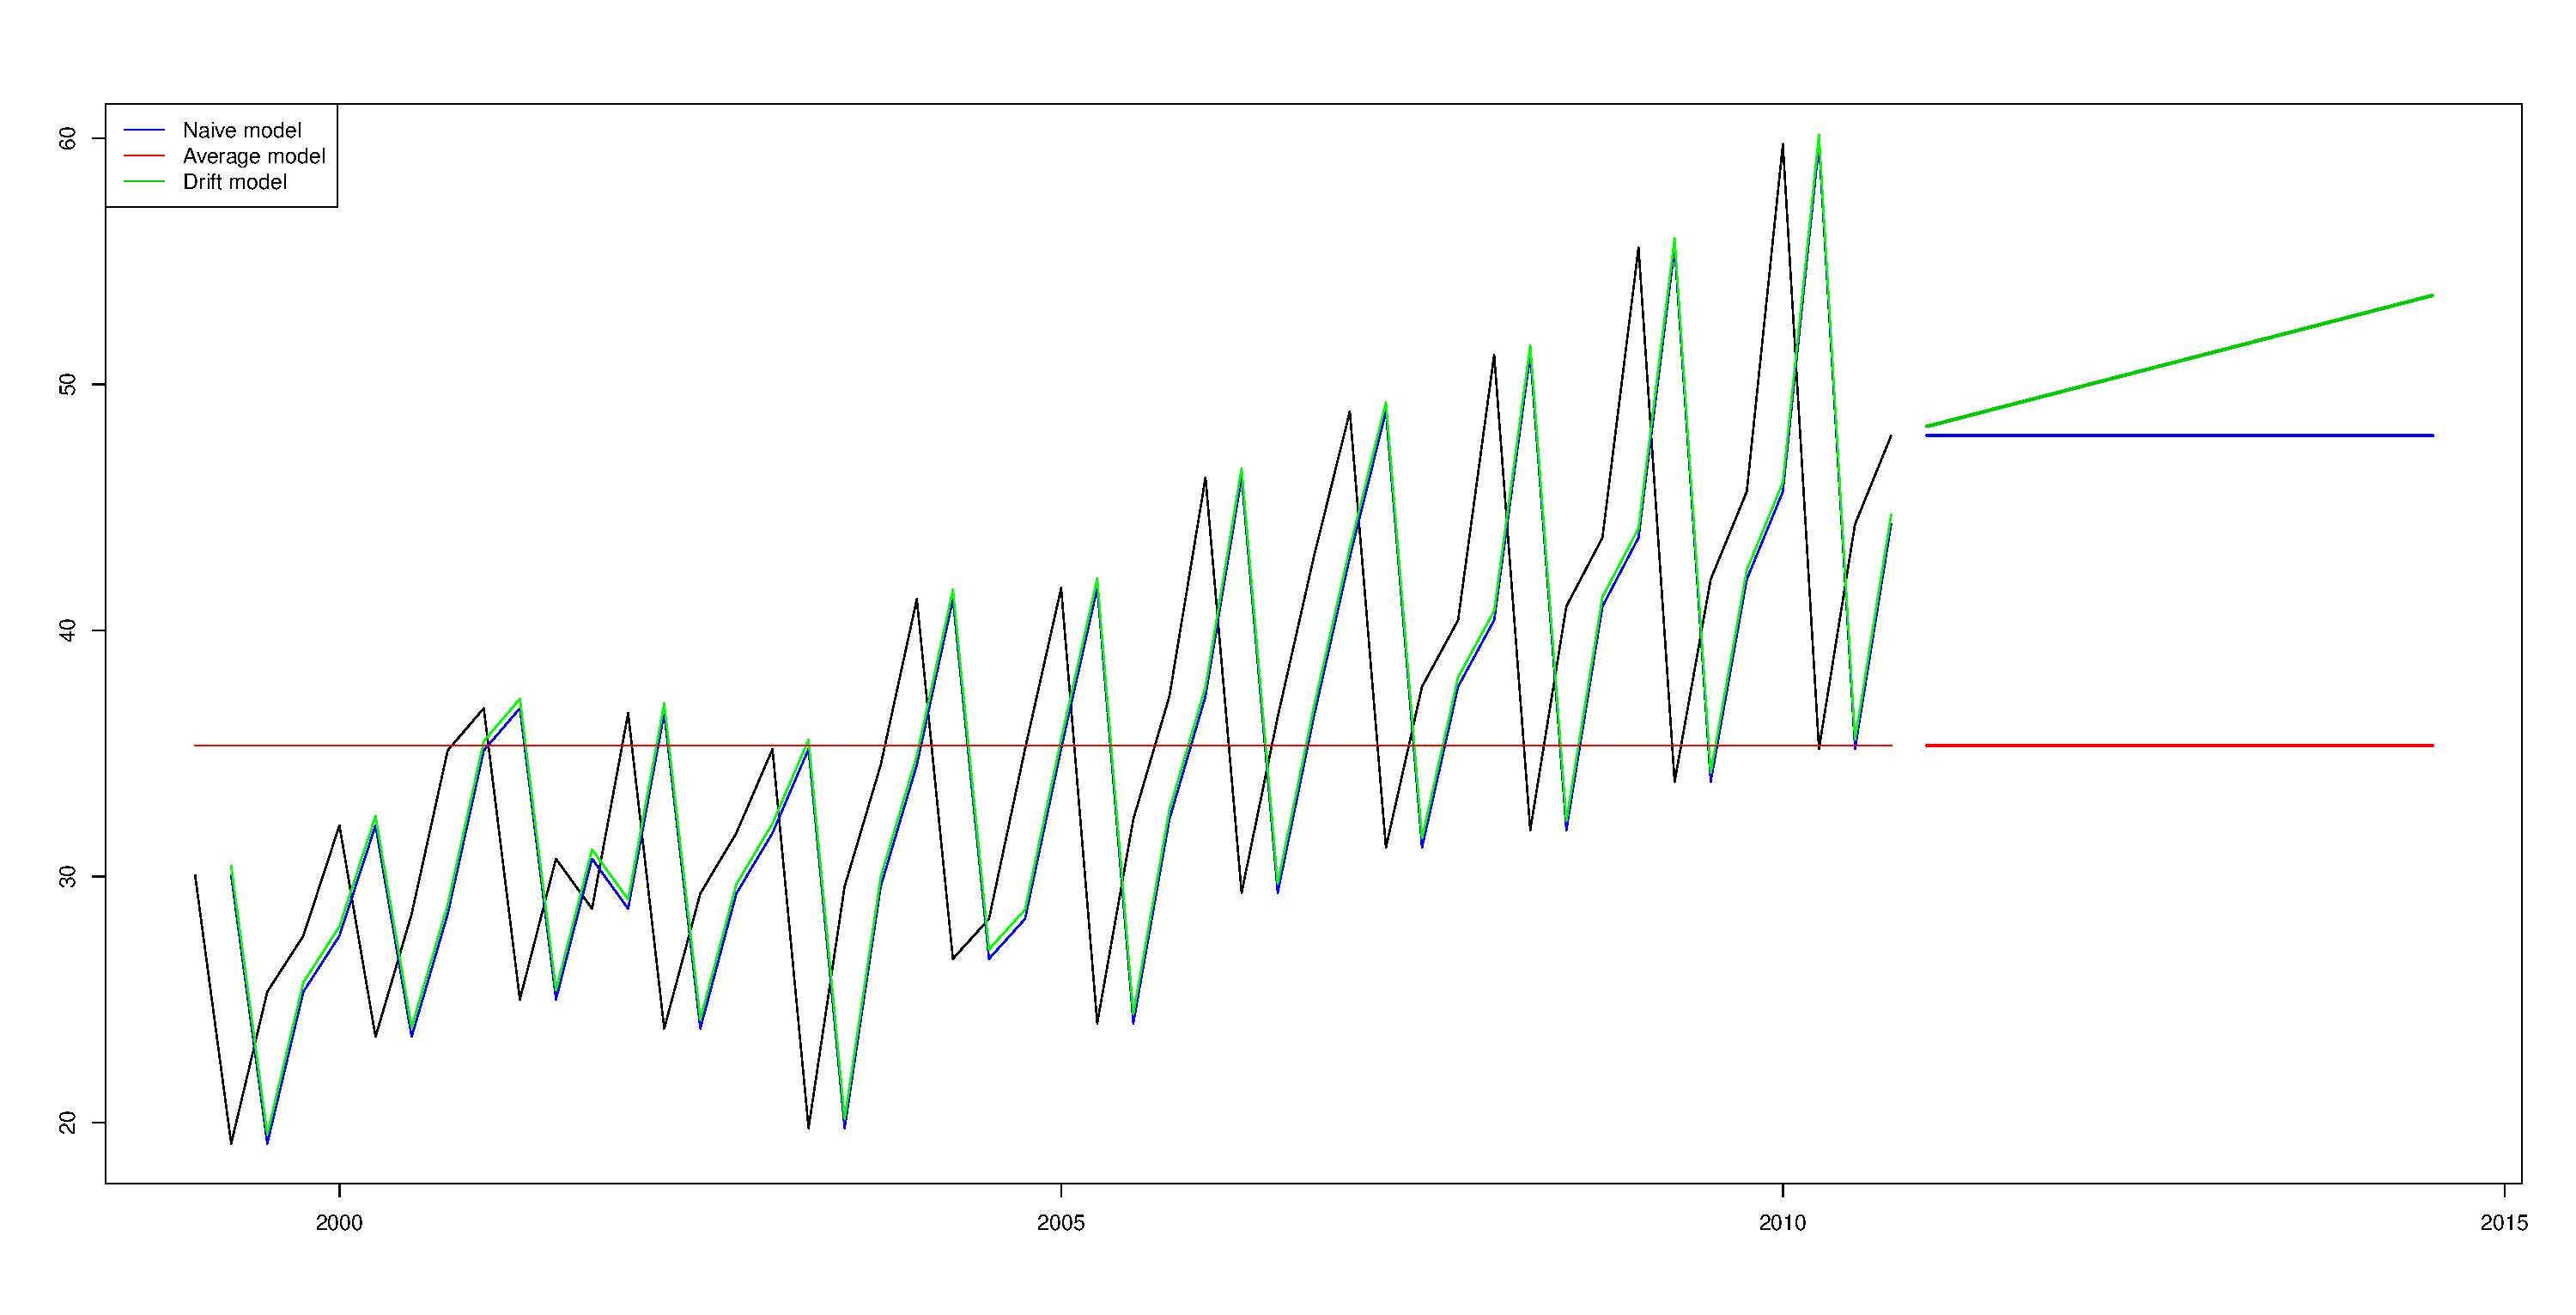
\includegraphics{img/simple-models.pdf}}
            \caption{Simple models on \emph{austourists}.}
            \label{img:simple-models}
        \end{center}
    \end{figure}

    \begin{figure}[H]
        \begin{center}
            \scalebox{0.25}[0.2]{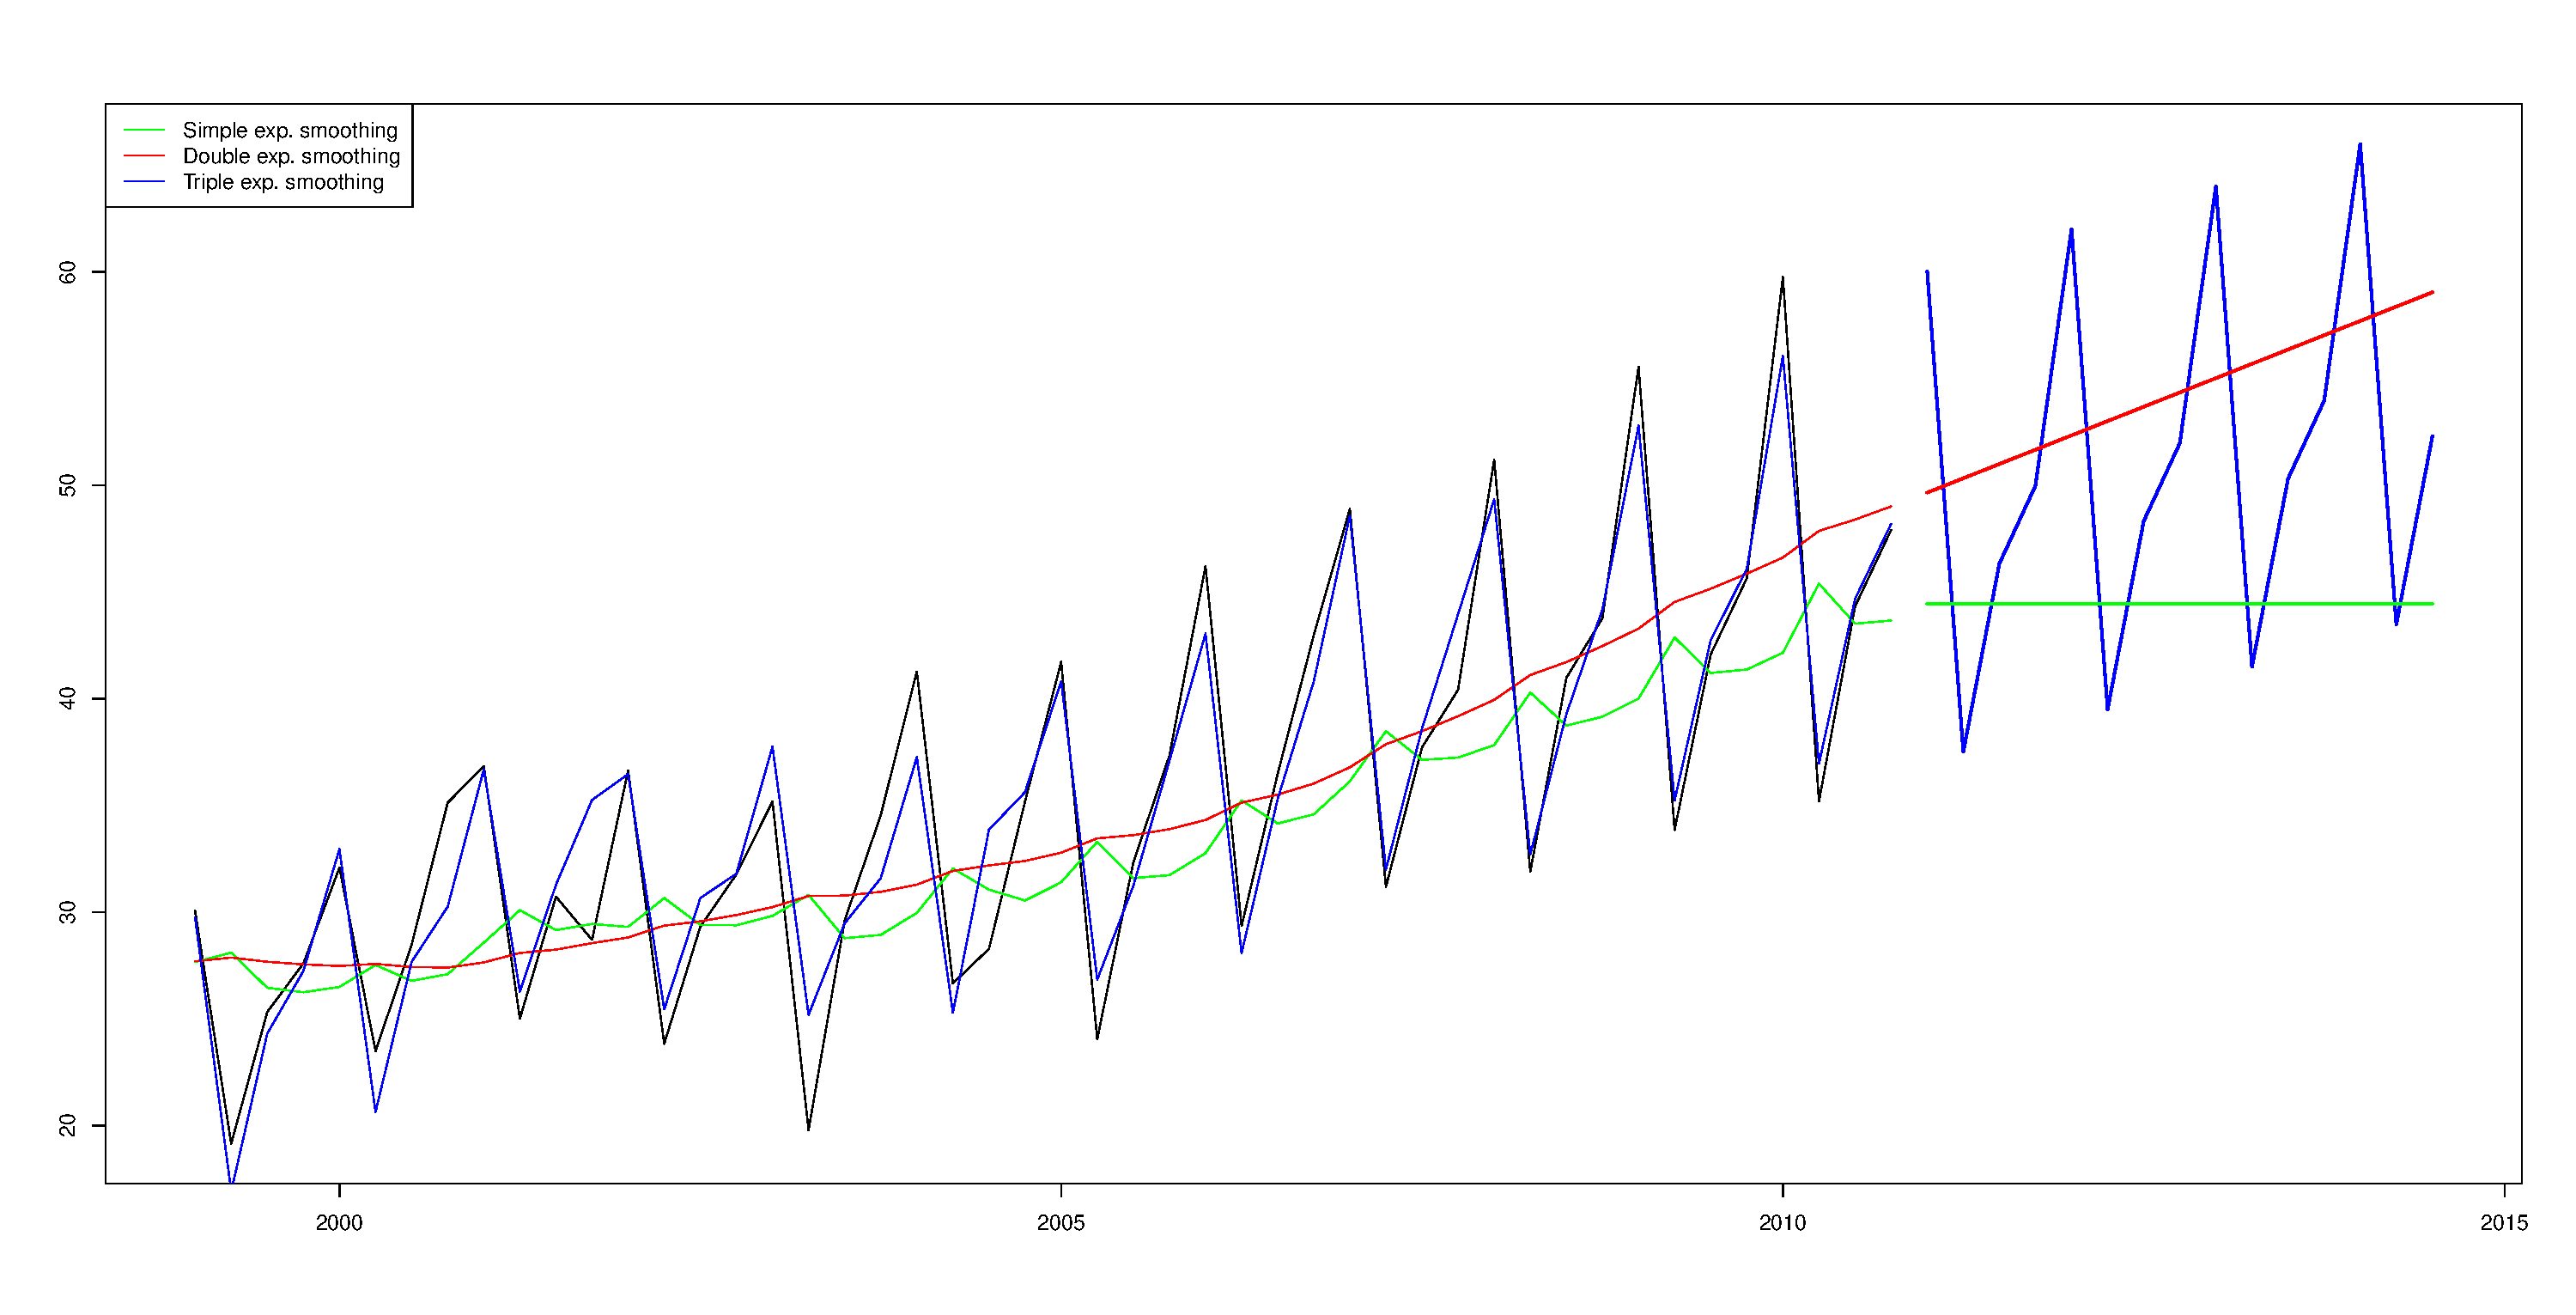
\includegraphics{img/exp-smoothings.pdf}}
            \caption{Exponential smoothings on \emph{austourists}.}
            \label{img:exp-smoothings}
        \end{center}
    \end{figure}

    \begin{figure}[H]
        \begin{center}
            \scalebox{0.25}[0.2]{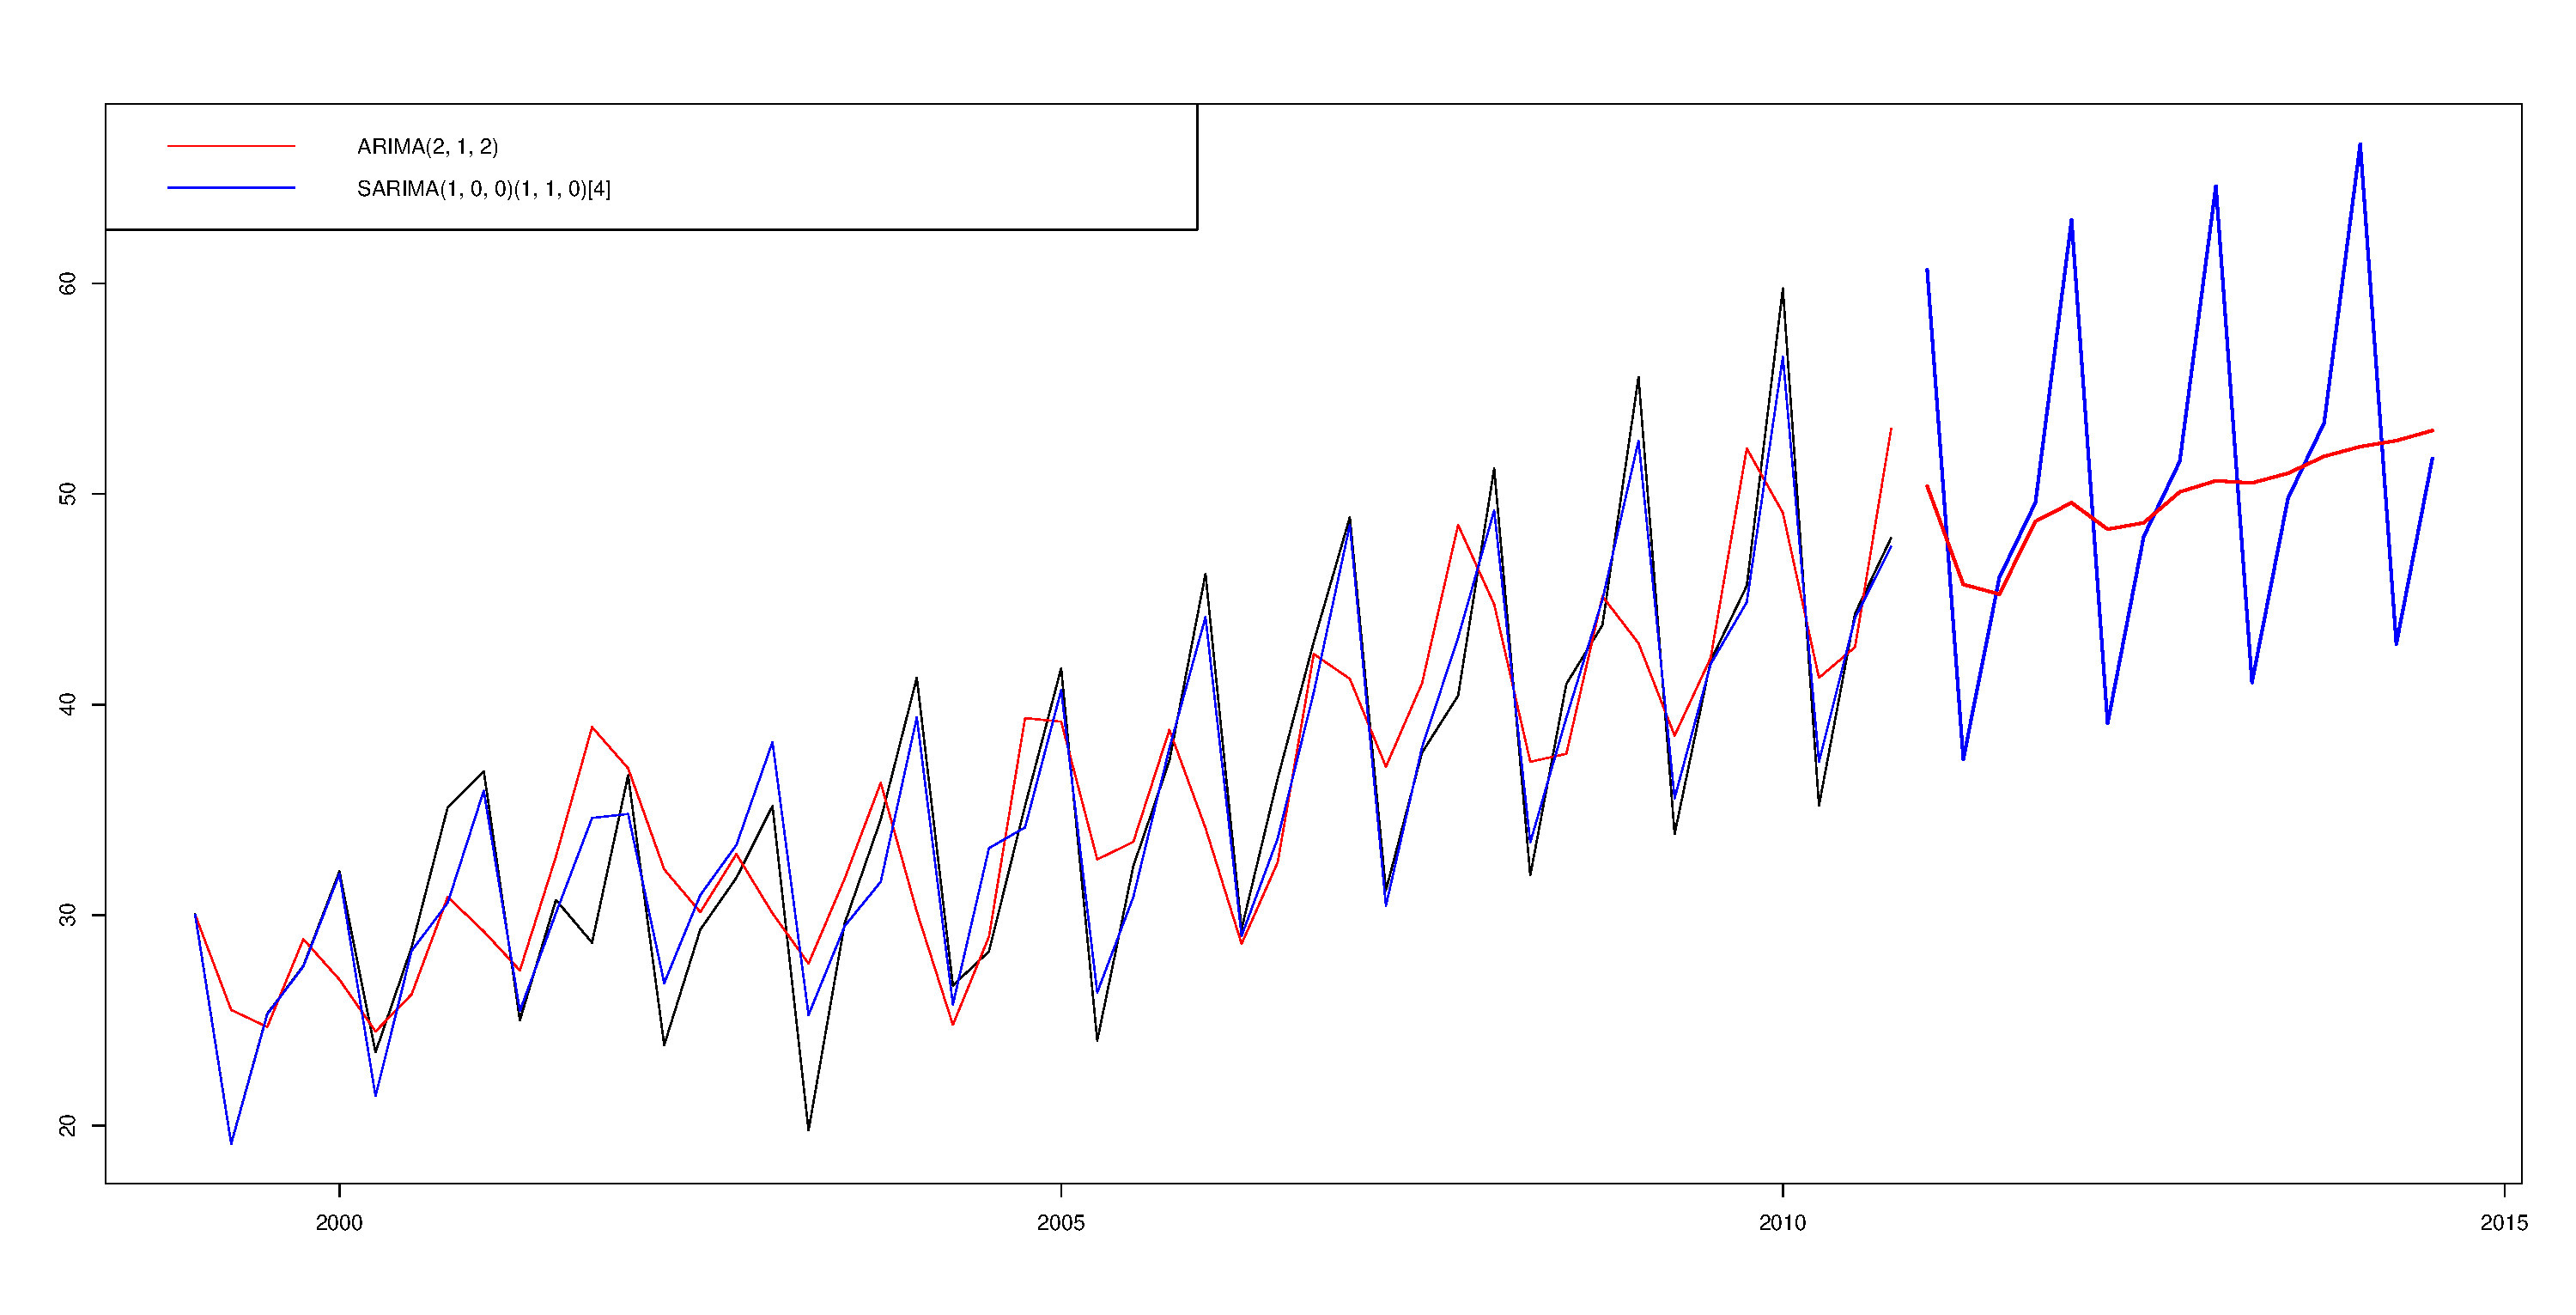
\includegraphics{img/arima-sarima.pdf}}
            \caption{Arima models on \emph{austourists}.}
            \label{img:arimas}
        \end{center}
    \end{figure}

    Exponential smoothings are depicted in \ref{img:exp-smoothings}. For this particular series it is obvious that
    seasonal is the best describing modelled time series. In the beginning can be seen how it the seasonal model
    changing and learning the seasonal pattern from data. Learning and adaptivity to new trends depends on smoothing
    parameters of the models. Higher values of parameters allows the model to quicier adapt to changes. Models with
    lower smoothing parameters are more robust to the changes.

    Arima models are showed in \ref{img:arimas}. Non seasonal model is already capable of capturing some seasonal
    patterns but it is more random whereas seasonal patterns should be of fixed period. Therefore seasonal Arima with
    dedicated model for each period is more appropriate.

    \begin{table}[h]
        \begin{center}
            \begin{tabular}{l|r|r|c}
                    \textbf{Model} & \textbf{MSE} & \textbf{MAE} & \textbf{AIC} \\ \hline \hline
                    Na\"{i}ve & 104.74 & 8.64 & \\
                    Drift & 104.60 & 8.47 & \\
                    Average & 79.91 & 7.14 & \\ \hline
                    Simple exp. smoothing & 53.54 & 5.91 & 380.88 \\
                    Double exp. smoothing & 44.41 & 5.28 & 375.90 \\
                    Triple exp. smoothing & 5.34 & 1.71 & 282.73 \\ \hline
                    Linear regression & 41.85 & 5.10 & 321.46 \\ \hline
                    ARIMA(2, 1, 2) & 30.88 & 4.35 & 310.6 \\
                    SARIMA(1, 0, 0)(1, 1, 0)[4] & 4.79 & 1.63 & 206.95 \\
            \end{tabular}
            \caption{Statistics of models.}
            \label{tab:models-stat}
        \end{center}
    \end{table}

    In \ref{tab:models-stat} are listed statistics produces by each model. Model with lowest one step ahead prediction
    is seasonal Arima and triple exponential smoothing which is correct for highly seasonal time series such as this
    one. For model selection would be used AIC statistics which is correlated to MSE.

%%%%%%%%%%%%%%%%%%%%%%%%%%%%%%%%%%%%%%%%%%%%%%%%%%%%%%%%%%%%%%%%%%%
\chapter{Existing Solutions}
Before directly going to the design and implementation let's briefly look at existing monitoring solutions and libraries
for time series modelling. In the next section are described not only direct competitors of Hawkular but also
generally available software of this kind. Because Hawkular is still only an upstream project and not deliverable
product for the customers thereby as alternative is considered Jboss Operations Network (JON). This work does not
focus on comparison of monitoring applications. It is mentioned for more wider overview of this domain and also
if some libraries can be used in the implementation.

    \section{Monitoring and Management Platforms}
    Out there are many monitoring solutions available. Some of them are offered as service (SaaS) and other need to be
    deployed in customer's environment. For each application are highlighted the most important features and how it
    differs from its rivals. It is also mentioned if the application offers predictive engine for metric data.

    \subsection{New Relic}
    New Relic was the first monitoring solution offered as SaaS \cite{new-relic}. It focuses on application performance
    rather than infrastructure view. Java applications monitoring is done by agent. Because agent manipulates
    with bytecote it is able to identify business transactions and monitor for instance utilization of REST endpoints
    Agent also automatically identifies databases connected to the application being monitored. From alert
    prediction perspective New Relic does not offer alert prediction or predictive charts.

    \subsection{Dynatrace Ruxit}
    Ruxit is another popular SaaS solution for monitoring middleware applications. Monitoring is also done by agents
    which instruments bytecode so the application is also able to monitor business transactions. Ruxit differs from
    others that it offers root cause analysis rather than firing multiple alerts. It directly shows causing problems
    with visual representation \cite{ruxit}. Ruxit does not offer predictive alerting or charts.

    \subsection{Open Source Projects}
    As Hawkular is an open source project it is important to mention it's direct competitors from this area. There are
    two major open source projects. The first one is Nagios and second Zabbix. Nagios was started in 1991 and Zabbix
    in 2001 therefore both are more than fifteen years old. By the time of writing this thesis last contribution to
    Nagios was from 17th September 2015 and Nagios project was active until the last moment. Both these projects does
    not offer alert prediction.

    \subsection{HP OpenView and IBM Tivoli}
    The biggest monitoring solutions offered by these two software giants are HP OpenView and IBM Tivoli. Both are
    composed of many independent products. Solution from HP does not offer any predictive capabilities.

    Operations Analytics, one of IBM Tivoli products can automatically detect correlations between
    metrics which can lead to detection of application issues, for example an anomaly detection. Another part of Tivoli
    solution\,--\,Netcool Network Management is capable of predicting events. There is also another predictive analysis
    in Tivoli Monitoring module\footnote{Available at \url{https://www.ibm.com/developerworks/community/wikis/home?lang=en\#/wiki/Tivoli+Monitoring/page/Details+for+ITPA+Predictive+Analytics+and+Non+Linear+Trending}}
    In the online document there is mentioned that predictive engine does not work on real time streams of data. Tivoli
    is definitely big solution and in order to get real predictive capabilities it would require to contact IBM
    support.

    \section{Libraries For Time Series Forecasting} \label{libraries-for-ts}
    In Java there is only one publicly available library for time series modelling. The library is called
    OpenForecast\footnote{Available at \url{http://www.stevengould.org/software/openforecast/index.shtml}}. It contains
    models like na\"{i}ve, linear regression and exponential smoothings. Whereas the library is open source, code
    was reviewed and tested. Some assumptions about the implementation were made. The parameters of some models are
    not estimated correctly. For example in linear regression slope and intercept are not estimated by minimizing
    sum of squared error.

    The library provides nice feature called automatic forecaster which selects the best model for given
    time series, however the code produces null pointer exception. The bug was identified but the library is no any more
    maintained.

    Performance of the library was also tested. Table \ref{tab:open-forecast-perf} contains execution times of
    simple, double and triple exponential smoothing models. The tested time series is generated sine function of
    length 200 observations. The result is compared against execution times of R's function \texttt{ets} from
    \texttt{forecast} package.

    \begin{table}[h]
        \begin{center}
            \begin{tabular}{l|c|c}
                \textbf{Model} & \textbf{OpenForecast} & \textbf{R \texttt{ets()} from \texttt{forecast}} \\ \hline \hline
                Simple ex. & 4.91 sec. & 0.003 sec.\\
                Double ex. & 9.31 sec. & 0.006 sec.\\
                Triple ex. & 6.45 sec. & 0.209 sec.\\
            \end{tabular}
            \caption{Execution time of parameters estimation for exponential smoothing models.}
            \label{tab:open-forecast-perf}
        \end{center}
    \end{table}

    From the table it is obvious that R's implementation is much faster. For example optimization of thousand double
    exponential smoothing models would take about two and half hour. This results are not acceptable for Hawkular in
    real time environment.

    Another possibility is to directly use R implementation. There are various libraries\footnote{The most widely used:
    RCaller and JRI}
    which allow executing R code from Java, however it requires installed R system in the target environment. Other
    possible solution is to use Rengin\footnote{Available at \url{http://www.renjin.org/}}\,--\,JVM interpreter for R.
    However \texttt{forecast} package depends on other package which allow native C++ invocation for optimized
    computations. Therefore package \texttt{forecast} can not be used with Rengin.

%%%%%%%%%%%%%%%%%%%%%%%%%%%%%%%%%%%%%%%%%%%%%%%%%%%%%%%%%%%%%%%%%%%
\chapter{Design and Implementation} \label{design-impl}
The module for an alert prediction is named Hawkular Data Mining. Source code is versioned in Git and
hosted on Github\footnote{Available at \url{https://github.com/hawkular/hawkular-datamining}} under
license Apache version 2.0.

The project is split into several Maven artifacts. This approach decomposes problem into smaller parts
which have dedicated functionality and can be easy reused in other projects. It also ensures that
third party dependencies are loaded only for certain artifacts where are needed. A figure \ref{appen:maven-deps}
shows dependency tree of \texttt{datamining-dist}, which is the top level artifact. The most important modules are
listed in \ref{tab:datamining-modules}. All of listed artifact ids have prefix \texttt{hawkular-datamining-}.

\begin{table}[h]
    \begin{center}
        \begin{tabular}{l|l}
            \textbf{Artifact Id} & \textbf{Description} \\ \hline \hline
            parent & Managing shared dependencies and versions. \\
            forecast & Core library for time series modeling and forecasting. \\
            api & Api used within Data Mining. \\
            rest & Web archive for standalone usage without Hawkular. \\
            dist & Web archive with Hawkular integration code. \\
            cdi & Support for context dependency injection. \\
            itest & Artifact for integration tests.
        \end{tabular}
        \caption{Hawkular Data Mining modules.}
        \label{tab:datamining-modules}
    \end{center}
\end{table}

In the following sections are described the most important parts of the implementation with respect to data structures
and used algorithms.

    %%%%%%%%
    \section{Design of Data Structures}
    The core data structures from \texttt{datamining-forecast} package are interfaces for time series models
    \ref{alg:models}and forecasters. This two interfaces are related but not the same. Each time series model should be capable of
    predicting and learning. The main difference between forecaster and time series model is that forecaster
    is designed for online learning and it autonomously selects the most appropriate time series model. Time series
    models by default are not designed for online learning, however it can be accomplished with a wrapper class.

    Metric in the Data Mining is represented as structure \texttt{MetricContex} which contains metadata like
    collection interval, metric id and tenant id. Collection interval is necessary for calculating timestamps of
    predicted points.

    \begin{lstlisting}[caption={Interface for time series models.}, language=Java, label={alg:models}]
interface TimeSeriesModel {
    void learn(List<DataPoint> ts);
    List<DataPoint> forecast(int steps);
    int numberOfParameters();
    MetricContext context();
    AccuracyStatistics initStatistics();
    AccuracyStatistics runStatistics();
    ...
     }
    \end{lstlisting}

    The next package is \texttt{api}. It depends on \texttt{forecast} and it eventually could
    depend on another library for data analysis, for instance a library for an outlier detection. In this package there
    is a code necessary for using Data Mining as a web application, for instance classes for accessing data analysis
    objects of given metric.

    The interface \texttt{SubscriptionManager} was designed for accessing time series analysis objects. Some of its
    methods are listed in \ref{alg:sub-manager}. Implementation of this interface could store entities in database.
    However, Data Mining directly does not use any database. Therefore \\ \texttt{SubscriptionManager} holds all objects
    in memory. Internally it stores objects in map where the key is tenant and value another map where the key is
    metric id and value finally the object for data analysis\,--\,\texttt{Subscription}.

    \begin{lstlisting}[caption={Interface \texttt{SubscriptionManager}.}, language=Java, label={alg:sub-manager}]
interface SubscriptionManager {
     void subscribe(Subscription, Owner);
     void unsubscribe(tenant, metric, Owner);
     Subscription model(tenant, metric);
     ...
     }
    \end{lstlisting}

    \texttt{Owner} specifies the owner who enabled prediction. The core class for data analysis is
    \texttt{Subscription}. Currently only time series forecasting is available.
    This object holds an instance of an automatic forecaster. Class diagram of the most important classes
    from \texttt{forecast} and \texttt{api} is in \ref{appen:class-diagram}.

    The build produces two web archives. The first one is designed for standalone usage and the second for deployment
    into Hawkular. Both uses forecasting capabilities from \texttt{api} and \texttt{forecaster}.
    REST api is implemented in \texttt{rest} and then reused in integration module \texttt{dist}.
    For REST api implementation the standard JAX-RS is used.

    Tests for REST api are in separate artifact \texttt{itest} which allows reusing them, for instance in the main
    integration project.

    Some of the service classes like \texttt{SubscriptionManager} are used in several other classes and also multiple
    implementation could exists (in memory or database implementation). Therefore dependency injection
    design pattern was introduced. Used technology is Java context dependency injection (CDI). In order to keep
    api classes clean module \texttt{cdi} with CDI configuration was introduced.

    %%%%%%%%
    \section{Automatic Forecaster}
    The most important class in Data Mining for doing predictions is \texttt{AutomaticForecaster} this class
    autonomously decides which time series model should be used for modelled time series. Currently it decides from
    three implemented models: simple, double and triple exponential smoothing. Other models which implement interface
    \texttt{TimeSeriesModel} can be easy added.

    The most importantly this class is capable of dealing with concept drift. It holds circular buffer of historical
    metrics and if statistical properties of underlying time series changes content of the buffer is used for selecting
    new model. The strategy when a new model should be selected is configurable. System currently supports two
    strategies. The first strategy periodically each $n$ observations selects new model.
    The Second one is more sophisticated and it selects a new model only when the error of learning one step
    ahead predictions exceeds by $x\%$ error calculated on learning points when model was selected.

    Model selection is based on information citerions from section \ref{model-selection}. Automatic forecaster in
    successive steps calls optimizers of given models and then selects the best with the lowest information criterion.
    Used criterion is configurable for each forecaster is configurable.

    %%%%%%%%
    \section{Model Optimizers} %TODO
    Model optimizers are the most important part of the model implementation. If the parameters of model are not
    estimated correctly model would produce high forecasting error. The idea behind optimization is to find the
    best parameters of the model that one step ahead forecasting error is the lowest possible. In general number of
    steps can be more than one. Formaly % TODO

    \begin{eqnarray} \label{likelihood}
da
    \end{eqnarray}

    Then well defined objective function for minimization is passed to non\,--\,linear optimization algorithm from
    Apache Math Commons. This library implements several optimization algorithms: Nelder-Mead simplex,
    Virginia Torczon's multi-directional and Mike Powell's BOBYQA. These algorithms does not need computed derivatives
    of the cost function.

    The best results were acquired from Nelder-Mead simplex algorithm. Criterions were optimization execution time and
    quality of the estimated parameters. Estimated parameters were compared to R's estimations.

    Table \ref{tab:open-forecast-perf} contains execution times comparison of \texttt{OpenForecast} and R
    implementation. This section addes execution time of Data Mining implementation. Complete execution times are
    listed in \ref{tab:datamining-perf}. Execution times of Data Mining's optimizers are in some cases faster than R.

    \begin{table}[h]
        \begin{center}
            \begin{tabular}{l|c|c|c}
                \textbf{Model} & \textbf{OpenForecast} & \textbf{R \texttt{ets()} from \texttt{forecast}} &
                    \textbf{Data Mining}\\ \hline \hline
                Simple ex. & 4.91 sec. & 0.003 sec. & 0.033 sec.\\
                Double ex. & 9.31 sec. & 0.006 sec. & 0.002 sec. \\
                Triple ex. & 6.45 sec. & 0.209 sec. & 0.023 sec. \\
            \end{tabular}
            \caption{Execution time of parameters estimation for exponential smoothing models.}
            \label{tab:datamining-perf}
        \end{center}
    \end{table}

    %%%%%%%%
    \section{Integration into Hawkular}
    As it was mentioned before the build produces two web archives, one for standalone usage and another for
    deployment into Hawkular. The second web archive adds extra functionality for interacting with other Hawkular
    components.

    Hawkular as a project is packaged as a modified Wildfly server with several Hawkular components
    deployed. In Hawkular all entities are stored in Inventory, therefore Data Mining uses this module
    for querying metrics definitions and it adds some extra attributes necessary for predictions. Another module
    which is used by Data Mining is Hawkular Metrics. It is a metric storage based on hybrid key-value
    database Apache Cassandra. Diagram \ref{img:hawkular-interaction} shows Data Mining integration into Hawkular.

    \begin{figure}[H]
        \begin{center}
            \scalebox{0.32}{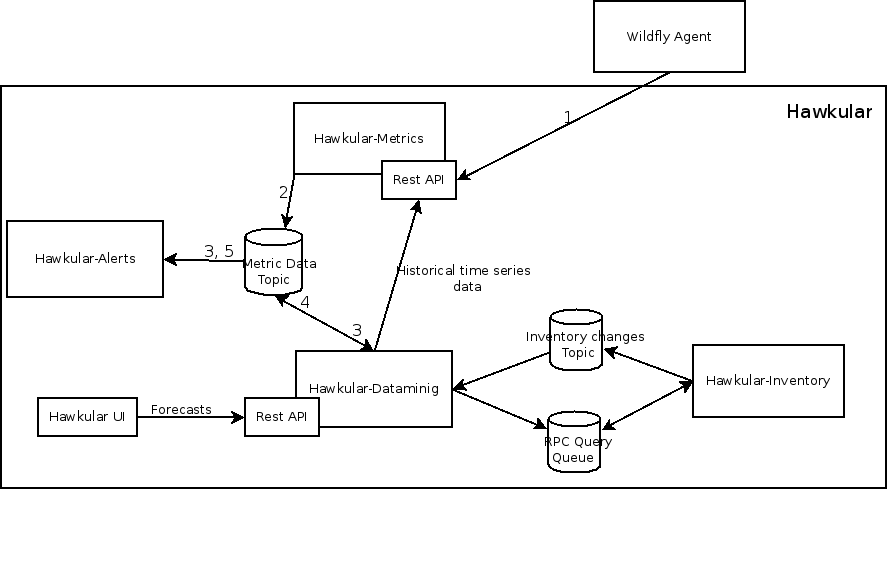
\includegraphics{img/src/architecture.pdf}}
            \caption{The integration into Hawkular.}
            \label{img:hawkular-interaction}
        \end{center}
    \end{figure}

    When Data Mining is deployed into Hawkular users can enable predictions by creating Relationship\footnote{Entity
    from Inventory which can be created between arbitrary two entities.} from tenant to the target entity. This target
    entity can be metric, metric type or tenant. When relationship is created from tenant to tenant predictions are
    enabled for all metrics under given tenant. Similarly, when a target entity is a metric type, predictions are
    enabled for all metrics of that type. In the figure \ref{img:relationship} is depicted part of the structure of
    inventory with enabled predictions.

    Relationships also stores properties needed for predictions. One of them is
    forecasting horizon which tells how many prediction steps are performed for each new incoming metric data
    points. With this approach of storing relationships in Inventory, Data Mining doesn't have to use any database for
    entities related to predictions. This approach was achieved without any changes to Inventory data
    model, this shows that Inventory's generic data model build on top of graph database\footnote{Compatible with
    Apache Tinkerpop} is good approach for storing data model in this domain.

    \begin{figure}[H]
        \begin{center}
            \scalebox{0.35}{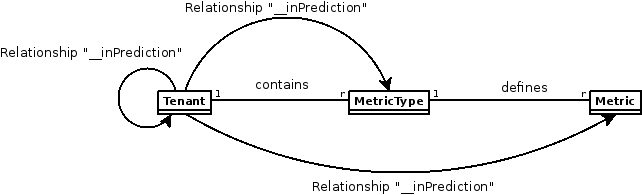
\includegraphics{img/src/inventory.pdf}}
            \caption{Relationship between entities of Inventory.}
            \label{img:relationship}
        \end{center}
    \end{figure}

    Any changes in Inventory are propagated to Data Mining by subscribing to specific events. This propagation is done
    through JMS topic where Inventory sends these events. However on application start Data Mining also needs to query
    all predictive relationships from inventory. For this purpose JMS request-response communication was implemented in
    Inventory. Any component which has access to internal messaging subsystem can construct query and send it for
    execution to Inventory. As solution REST api was also proposed but it could expose vulnerability\,--\,client
    could access any data objects of any tenant. Diagram \ref{img:sequence-enab-pred} depicts sequence of calls when
    prediction gets enabled.

    From the diagram \ref{img:sequence-enab-pred} is clear that when a prediction gets enabled historical metrics are
    queried from Metrics module. This means that Data Mining needs access to metrics of all tenants. It is the similar
    scenario like getting all predictive relationships from Inventory. It could not be implemented via REST api
    because of potential vulnerability and JMS based query was also rejected by Metrics owners.

    Another two solutions were proposed. The first was to bypass Metrics and query data directly from Cassandra.
    The second was inject Metrics as CDI bean and use its Java api. The first solution was refused because the schema
    is maintained by Metrics and can eventually can change also the backed (Cassandra) can change. The final
    solution which is also implemented is injecting Metrics as CDI bean. This solution assumes that Metrics
    are deployed in the same application server as Data Mining. From the performance perspective it is faster that
    JMS or REST calls.

    \begin{figure}[H]
        \begin{center}
            \scalebox{0.30}[0.20]{\includegraphics[angle=0]{img/src/uml-enable-predictions-sequence.pdf}}
            \caption{Sequence diagram of enabling predictions.}
            \label{img:sequence-enab-pred}
        \end{center}
    \end{figure}

    Diagram \ref{img:sequence-incoming-data} shows complete data flow from agent to alerts evaluation engine.
    Metric data is sent by agent to Metrics REST endpoint and stored in database. Then it is sent to JMS topic and
    consumed by Alerts and Data Mining. In parallel Alerts evaluates alerts criteria and Data Mining computes
    predictions. After computation predicted data are sent to the same JMS topic and consumed by Alerts.

    Data Mining changes \texttt{id} of predicted points in order to be able to distinguish original time series from
    predicted. For predicted metrics Alerts can evaluate the same conditions as for original time series or use
    different ones. At this point an alert for predicted metrics can be triggered.

    \begin{figure}[H]
        \begin{center}
            \scalebox{0.33}[0.24]{\includegraphics[angle=0]{img/src/uml-incoming-data-sequence.pdf}}
            \caption{Sequence diagram of incoming data from agent.}
            \label{img:sequence-incoming-data}
        \end{center}
    \end{figure}

    %TODO metric Explorer section

    %%%%%%%%
    \section{Test Automation and Documentation}
    Core functionality of the application is covered by unit tests. Junit framework is used for this type of tests.
    Because Data Mining interacts with other applications and modules integration tests are also implemented. These
    tests are run from Maven profile which starts web server with necessary modules deployed.
    Last type of implemented tests are end-to-end tests which calls REST endpoint of one module and expect result
    in call from another module. This type of tests are also executed in Maven profile with running web server.
    End-to-end tests for Data Mining project live in the main Hawkular integration repository\footnote{
    Available at \url{https://github.com/hawkular/hawkular}.}.

    All tests are automatically executed every time developer creates a pull request or pushes code to the master
    branch. For this Travis continuous integration platform was used which is for free for open source projects on
    Github.

    Documentation is directly written in Java code as javadoc. REST api documentation is also directly
    written in source code using Swagger framework and automatically generated at build time
    \footnote{Available at \url{http://www.hawkular.org/docs/rest/rest-datamining.html}}.

    %%%%%%%%
    \section{Releases}
    By the time writing of this thesis there was only one release with version \texttt{0.1.Final}. It is also available
    in the Maven central repository. Complete group id is \texttt{org.hawkular.datamining}. The most important
    artifact ids are listed in \ref{tab:datamining-modules}. Release notes of the release are available on
    Github\footnote{Available at \url{https://github.com/hawkular/hawkular-datamining/releases}}.

    \section{Retrospective}
    % TODO

%%%%%%%%%%%%%%%%%%%%%%%%%%%%%%%%%%%%%%%%%%%%%%%%%%%%%%%%%%%%%%%%%%%
\chapter{Evaluation of Implemented Models}
%TODO
TODO Do an example how to generate an alert.

    %%%%%%%%
    \section{Prediction capabilities}
    Show prediction capabilities of implemented models.
    TODO Can I compare it against R implementation?

    %%%%%%%% 
    \section{The Most Important Metrics}
    %TODO 
    TODO select subset of the most important metrics and show on them predictions.

%%%%%%%%%%%%%%%%%%%%%%%%%%%%%%%%%%%%%%%%%%%%%%%%%%%%%%%%%%%%%%%%%%% 
\chapter{Conclusion}

